


To pass the dispersive bounds on the differentiated field $\epsilon'$ back onto the error $\epsilon$, we need to prove appropriate non-linear elliptic estimates for non-linear Cauchy-Riemann operator relating the two fields via \eqref{hasimoto3}, i.e. we study the equation 
    \begin{equation}\label{eq:CR3}
        \epsilon' 
            =\partial_{\overline z} u ,
    \end{equation}
where the Cauchy-Riemann operator acts on $m$-equivariant fields by 
    \[
        \partial_{\overline z} u 
            := \partial_r u - \frac{m}{r} u \times Ru.
    \]
Recall the linearised operator takes the form   
    \[
        \mathsf L_u \phi 
            :=  u_1 \partial_r {u_1}^{-1}.
    \]

\subsection{Linearised equation}

To identify the main terms, we linearise the equation by decomposing the error into a component perpindicular to the soliton profile (i.e. in the tangent space $T_Q \SS^2$) and a component parallel to the soliton profile, 
\begin{equation}\label{eq:perpparallel}
    \begin{split}
        u(t, r) 
            &=  \underbrace{Q(r)}_{\text{soliton profile}} + \underbrace{\epsilon(t, r)}_{\text{perturbation}} \\
            &= \underbrace{Q(r)}_{\text{soliton profile}} + \underbrace{u_{\mathrm{lin}} (t, r)}_{\text{perpindicular perturbation}} + \underbrace{\gamma(t, r) Q(r)}_{\text{parallel perturbation}}
    \end{split}
\end{equation}
For the more visually-inclined reader, see Figure \ref{fig:decomp} below, 

\begin{figure}[h]
\begin{center}
    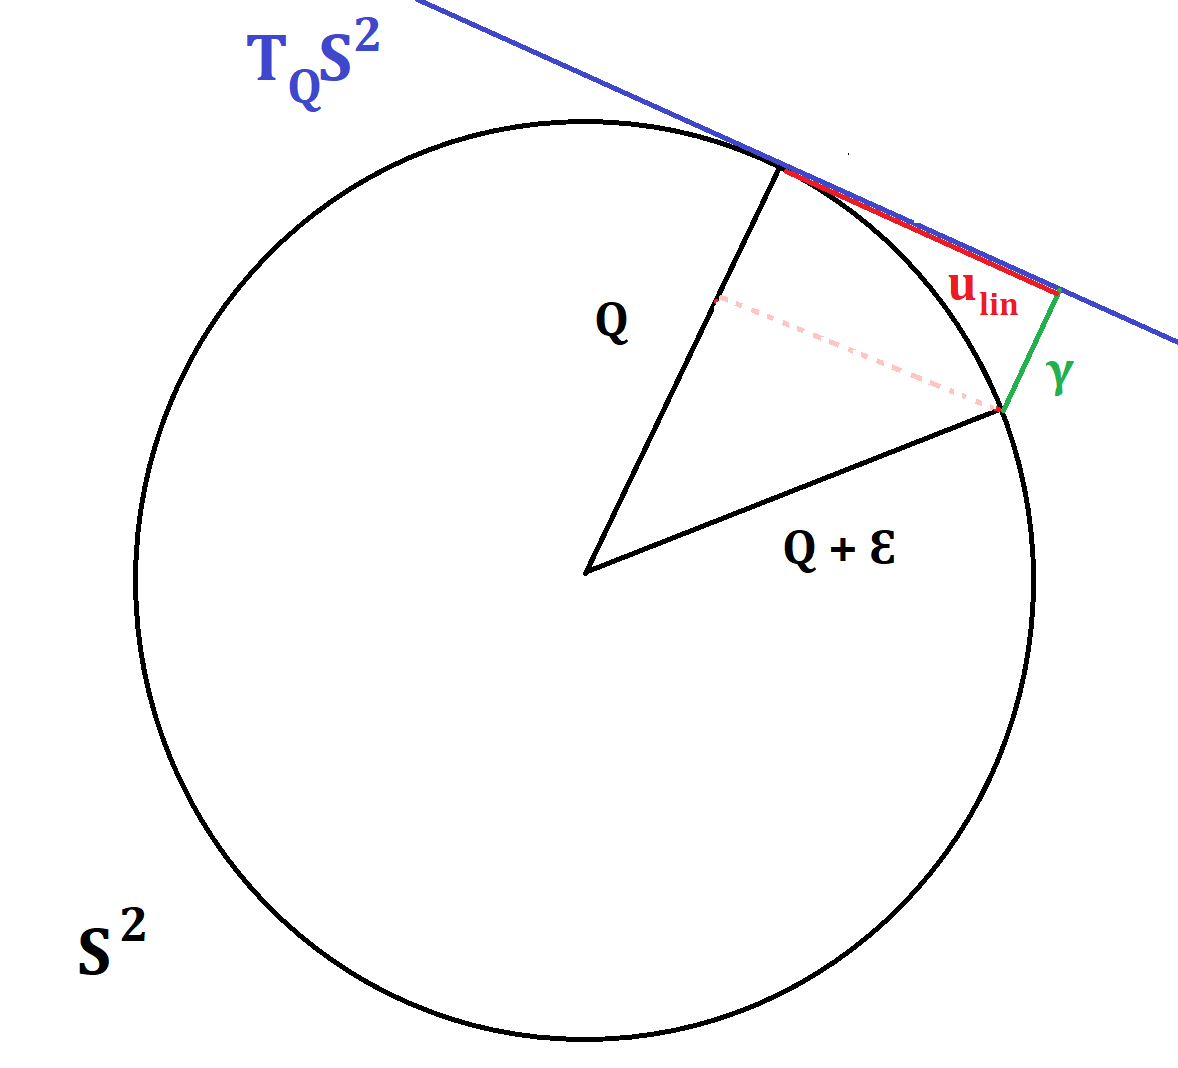
\includegraphics[scale = 0.3]{graphics/coulombQ}
    \caption{Decomposition of the error 
        \[\epsilon = u_{\mathrm{lin}} + \gamma Q,\] 
    into a component parallel to the soliton $\gamma Q \in \operatorname{span} Q$ and a component in the tangent space $u_{\mathrm{lin}} \in T_Q \SS^2$. For small error, the main term is the latter. }\label{fig:decomp}
\end{center}
\end{figure}

For small perturbation $|\epsilon| \ll 1$, the main term in the decomposition \eqref{perpparallel} is the perpindicular component $\epsilon \approx u_{\mathrm{lin}}$ in view of the constraint $|u| \equiv |Q| \equiv 1$; indeed one can compute that the parallel part is of quadratic order in $\epsilon$, 
\begin{align*}
    \gamma 
        &= \sqrt{1 - |u_{\mathrm{lin}}|^2} - 1 = O(|u_{\mathrm{lin}}|^2).
\end{align*}
Analogous to the study of the dispersive equation \eqref{hasimoto2}, we would like to fix a coordinate system which reveals the elliptic structure of the equations \eqref{hasimoto3} and furthermore is well-adapted to the decomposition \eqref{perpparallel}. In this case, we choose the Coulomb frame $\{\vec v_Q, \vec w_Q \} \subseteq Q^* T\SS^2$ adapted to the soliton profile $Q$, which takes the explicit form 
\begin{equation}\label{eq:coulombQframe}
        \vec v_Q (r) 
            = \begin{pmatrix} h_3 (r) \\ 0 \\ - h_1 (r) \end{pmatrix},
        \qquad
        \vec w_Q (r) 
            = \begin{pmatrix} 0 \\ 1 \\ 0 \end{pmatrix}. 
\end{equation}
In these coordinates, the fields $u_{\mathrm{lin}} : I \times \R^2 \to Q^* T\SS^2$ and differentiated field $\epsilon' : I \times \R^2 \to u^* T\SS^2$ correspond respectively to the complex scalar fields $\phi : I \times \R^2 \to \C$ and $\widetilde{\psi} : I \times \R^2 \to \C$, defined by 
    \begin{align*}
        \phi
            &:= \big\langle  u_{\mathrm{lin}}, \vec v_Q \big\rangle + i \big\langle u_{\mathrm{lin}}, \vec w_Q \big\rangle,\\
        \widetilde{\psi} 
            &:= \big\langle  \epsilon' , \vec v_Q \big\rangle + i \big\langle \epsilon', \vec w_Q \big\rangle.
    \end{align*}
Using the decomposition \eqref{perpparallel}, we can write the  inhomogeneous Cauchy-Riemann equation \eqref{CR3} in the Coulomb frame as 
\begin{equation}\label{eq:CRcoulomb}
    \underbrace{\mathsf L_Q \phi}_{\text{linearised operator}} 
        = \underbrace{\widetilde{\psi}}_{\text{dispersive bound}} - \underbrace{\frac{m}{r} \epsilon_3 \phi + \frac{m}{r} h_1 \gamma}_{\text{perturbative non-linearity}}. 
\end{equation}    
Thus, we see that, at least on the linear level, passing bounds on the differentiated field $\widetilde{\psi}$ to the main error $\phi$ amounts to inverting the linearised operator $\mathsf L_Q$. 

\subsection{Elliptic estimates}

The right-inverse is given by 
    \[
        \mathsf R_\chi g (r) 
            := 2\pi h_1 (r) \int_0^\infty \left( \int_{r'}^r h_1(r'') g(r'') dr'' \right) \overline{\chi (r')} h_1 (r') \, r' dr'.  
    \]

\begin{lemma}[Linear elliptic estimate]\label{lem:linearelliptic}
    For each $\lambda > 0$ and radial function $\chi : (0, \infty) \to (0, \infty)$, there exists a linear operator $\mathsf R_{\lambda, \chi}$ which serves as a right-inverse for $\mathsf L^\lambda$ and also a left-inverse for $\mathsf L_{\lambda}$ modulo the kernel, 
        \begin{align}
            \mathsf L^\lambda \mathsf R^\lambda_{\chi} g 
                &= g, \\
            \mathsf R^\lambda_{\chi} \mathsf L^\lambda g
                &= g - h_1 (r/\lambda) \int_0^\infty g (r')\overline{\tfrac{1}{\lambda^2} \chi \big( \tfrac{r}{\lambda}\big)} r' dr'.
        \end{align}
Furthermore, for $1 \leq p \leq \infty$ and $|\theta| < m$, if $\chi \in r^{-1} (\ell^{p'} L^1)_x (0, \infty)$, then the right-inverse satisfies the bound
        \begin{equation}
            || r^{-\theta} \mathsf R^\lambda_{\chi} g ||_{(\ell^p L^\infty)_x} 
                \lesssim || r^\theta \chi||_{ (\ell^{p'}L^1)_x} || r^{-\theta - 1}g||_{ (\ell^p L^1)_x}
        \end{equation}
\end{lemma}

\begin{proof}
    Note that 
        \[
            g(r) 
                \mapsto g\big(\tfrac{r}\lambda\big), \qquad
            \chi(r) 
                \mapsto \tfrac{1}{\lambda^2} \chi \big( \tfrac{r}{\lambda}\big)
        \]
    are adjoint operators, so it suffices to prove the result for $\lambda = 1$. For the details, we refer the reader to \cite[Section 10.1]{GustafsonEtAl2010}. 
\end{proof}

\begin{proposition}[Non-linear elliptic estimates]
    For $m \geq 2$, consider the inhomogeneous non-linear Cauchy-Riemann equation \eqref{CRcoulomb}. If the error satisfies the orthogonality condition 
        \begin{equation}\label{eq:ellipticorthogonal}
            \int_0^\infty \phi (r) \overline{\widetilde{h_1}(r/\lambda)} \, r dr 
                = 0,
        \end{equation}
    where $\widetilde{h_1} \in C^\infty_c (0, \infty)$ is a smooth compactly-supported radial function satisfying $\langle h_1, \widetilde{h_1} \rangle_{L^2_r} = 1$, then 
        \begin{enumerate}
            \item $L^2_x$-type bound 
                \begin{equation}
                    ||\phi||_{\dot H^1_m}    
                        \lesssim || \psi ||_{L^2_r} + ||\phi||_{L^\infty_r} ||\phi||_{\dot H^1_m}, \label{eq:ellipticenergy}
                \end{equation}

            \item $L^\infty_x$-type bound
                \begin{equation}
                    ||r^{-1} \phi ||_{(\ell^p L^\infty)_r} 
                        \lesssim ||\psi ||_{L^\infty_r} + ||\phi||_{L^\infty_r} ||\phi||_{(\ell^p L^\infty)_r}.\label{eq:ellipticuniform}
                \end{equation}
        \end{enumerate}
 \end{proposition}

\begin{proof}
    By the orthogonality condition \eqref{ellipticorthogonal}, we have 
        \[
            \phi 
                = \mathsf R_{\lambda, \widetilde{h_1}} \mathsf L^\lambda \phi. 
        \]
    The equation \eqref{CRcoulomb} schematically takes the form 
        \[
            \mathsf L_Q \phi  
                = \widetilde{\psi} + O(|\phi|^2).
        \]
    Using the estimates from Lemma \ref{lem:linearelliptic} and the triangle inequality, placing one factor of $\phi$ in the non-linearity in $L^\infty_r$-norm and the other in either $\dot H^1_m$-norm or $(\ell^p L^\infty)_r$-norm, furnishes the $L^2_x$-bound and $L^\infty_x$-bound respectively. 
\end{proof}


\begin{proposition}[Hardy-Sobolev inequality]
    Let $m \geq 1$ and suppose $\phi \in \dot H^1_m (0, \infty)$ is $m$-equivariant, then 
        \begin{equation}
            ||\phi||_{L^\infty_r}
                \lesssim ||\phi||_{\dot H^1_m}\label{eq:elliptichardy}.
        \end{equation}
\end{proposition}

\begin{proof}
    Fundamental theorem of calculus and Cauchy-Schwartz. 
\end{proof}